\section{NetKAT}

\begin{frame}{NetKAT}
    \begin{itemize}
        \item A network programming language with a sound and complete
              equational theory
        \item An instance of the Kleene algebra with tests
        \item Programs are compiled to flow tables of OpenFlow switches
        \item A packet $pk$ is a record with fields $f_1,...,f_k$ 
    mapping to fixed-width integers 
    \end{itemize}
    \vspace{\baselineskip}
    NetKAT Syntax:
    \begin{align*}
        a,b ::= & 1 ~|~ 0 ~|~ f = n ~|~ a + b ~|~ a \cdot b ~|~ \neg a  \\
        p,q ::= & a ~|~ f \la n ~|~ p + q ~|~ p \cdot q ~|~ p^* ~|~ dup
    \end{align*}
\end{frame}

\begin{frame}{NetKAT: Example}
    \begin{figure}
        \centering
        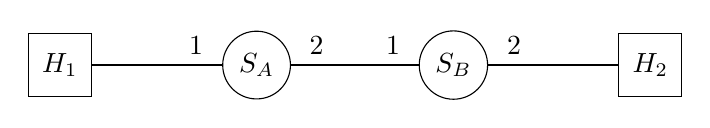
\begin{tikzpicture}[
                node distance={25mm},
                sw/.style = {draw, circle,minimum size=8mm},
                h/.style = {draw, rectangle,minimum size=8mm}
            ]
            \node[h] (h1)  {$H_1$};
            \node[sw] (sa) [right of=h1]  {$S_A$};
            \node[sw] (sb) [right of=sa] {$S_B$};
            \node[h] (h2)  [right of=sb] {$H_2$};
            \draw [thick] (h1)  -- node[above,pos=0.8]{1} (sa);
            \draw [thick] (sa) -- node[above,pos=0.2]{2}
            node[above,pos=0.8]{1}(sb);
            \draw [thick] (sb) -- node[above,pos=0.2]{2} (h2);
        \end{tikzpicture}
    \end{figure}

    Network Program in NetKAT:
    \begin{equation*}
        in \cdot (p_{AC}\cdot t)^* \cdot out
    \end{equation*}
    \begin{align*}
        in     & \triangleq (sw = A \cdot pt = 1) + (sw = B \cdot pt = 2)          \\
        p      & \triangleq (dst = H_1 \cdot pt \la 1) +
        (dst = H_2 \cdot pt \la 2)                                                 \\
        p_{AC} & \triangleq \neg(typ = SSH)\cdot p                                 \\
        t      & \triangleq  (sw = A \cdot pt = 2 \cdot sw \la B \cdot pt \la 1) + \\
               & (sw = B \cdot pt = 1 \cdot sw \la A \cdot pt \la 2) +             \\
               & (sw = A \cdot pt = 1) +                                           \\
               & (sw = B \cdot pt = 2)                                             \\
        out & \triangleq in
    \end{align*}
\end{frame}

\begin{frame}{NetKAT: Formal Reasoning}
    To establish that $p_{AC}$ filters SSH packets from $H_1$ to $H_2$:
    \begin{equation*}
        \begin{pmatrix}
            type = SSH \cdot sw = A \cdot pt = 1 \cdot \\
            (p_{AC}\cdot t) ^ * \cdot                  \\
            sw = B\cdot pt = 2
        \end{pmatrix}
        \equiv 0
    \end{equation*}
    \vspace{\baselineskip}
    To establish that $p_{AC}$ correctly forwards non-SSH packets from 
    $H_1$ to $H_2$:
    \begin{equation*}
        \begin{pmatrix}
            \neg(type = SSH) \cdot sw = A \cdot pt = 1 \cdot & \\
            sw \la B \cdot pt \la 2                          &
        \end{pmatrix}
        \leq (p_{AC}\cdot t)^ *
    \end{equation*}
\end{frame}